% -*- mode: LaTeX; mode: auto-fill; mode: flyspell; coding: utf-8; -*-
\documentclass[ucs]{beamer}
\usepackage[T2A]{fontenc}
\usepackage[english,russian]{babel}
\usepackage[utf8x]{inputenc}
\usepackage{verbatim}
\newenvironment{code}{\small\verbatim}{\normalsize\endverbatim}

\usetheme % [secheader]
    {Madrid}

\title[Управление памятью]{Статические политики восстановления памяти}
\author{Меринов Николай}
\institute{УрФУ}
\date{2012}
\begin{document}

\begin{frame}
  \begin{beamercolorbox}[ht=2.5ex,dp=1ex,center,rounded=true,shadow=true]%
    {frametitle}
    \usebeamerfont{frametitle}
    Статические политики восстановления памяти.
  \end{beamercolorbox}
  % Author and supervisor
  \begin{flushright} \large
    \emph{Автор:} \\
    студент гр. МГКН-2\\
    Меринов Николай Дмитриевич\\\ \\
    \emph{Научный руководитель:} \\
    старший преподаватель\\
    Лукач Юрий Саулович
  \end{flushright}
  \vfill
  \begin{center}
    {2012}
  \end{center}
\end{frame}

\begin{frame}[fragile]
  \frametitle{Политики управления памятью.}
  \framesubtitle{}
  %% написать
  \begin{block}{Определения}
    \begin{itemize}
    \item Политика --- общее руководство для действий и принятия решений,
      которое облегчает достижение целей. %policy
    \item Выделение памяти --- предоставление программе памяти доступной для
      хранения программы.
    \item Восстановление памяти --- возвращение ранее выделенной памяти
      менеджеру памяти.
    \end{itemize}
  \end{block}
\end{frame}

\begin{frame}[fragile]
  \frametitle{Статическое выделение памяти.}
  \framesubtitle{}
  \begin{block}{Плюсы}
    \begin{itemize}
    \item Предсказуемость потребление памяти.
    \item Простота реализации.
    \end{itemize}
  \end{block}

  \begin{block}{Минусы}
    \begin{itemize}
    \item Невозможны структуры переменных размеров.
    \item Невозможно создание рекурсивных процедур.
    \item Невозможно создать новые структуры в процессе работы.
    \end{itemize}
  \end{block}
\end{frame}

\begin{frame}[fragile]
  \frametitle{Выделение памяти на стеке.}
  \framesubtitle{}
  \begin{block}{Плюсы}
    \begin{itemize}
    \item Предсказуемость потребление памяти.
    \item Возможность создания рекурсивных процедур.
    \item Локальные данные переменного размера.
    \end{itemize}
  \end{block}

  \begin{block}{Минусы}
    \begin{itemize}
    \item Невозможно вернуть в качестве результата данные переменного размера.
    \item Срок жизни активационной записи функции ограничен временем работы
      функции её вызвавшей.
    \end{itemize}
  \end{block}
\end{frame}

\begin{frame}[fragile]
  \frametitle{Выделение памяти в куче.}
  \framesubtitle{}
  \begin{block}{Плюсы}
    \begin{itemize}
    \item Размер данных может определяться во время исполнения.
    \item Время жизни данных может быть больше чем время жизни объектов их
      создавших.
    \end{itemize}
  \end{block}

  \begin{block}{Минусы}
    \begin{itemize}
    \item Для восстановления памяти требуется отдельная политика.
    \end{itemize}
  \end{block}
\end{frame}

\begin{frame}[fragile]
  \frametitle{Выделение памяти на стеке регионов.}
  \framesubtitle{}
  \begin{block}{Плюсы}
    \begin{itemize}
    \item Размер данных может определяться во время исполнения.
    \item Возможно возвращение из функции данных переменного размера.
    \item Существует естественная политика восстановления памяти.
    \end{itemize}
  \end{block}

  \begin{block}{Минусы}
    \begin{itemize}
    \item Ослабление контроля срока жизни данных.
    \item Без дополнительных усилий при разработке программы данные
      ``стекаются'' в регионы на нижних уровнях стека и существуют намного
      дольше необходимого.
    \end{itemize}
  \end{block}
\end{frame}

\begin{frame}[fragile]
  \frametitle{Восстановление памяти на куче.}
  \framesubtitle{}
  \begin{block}{Политики}
    \begin{itemize}
    \item Ручное управление памятью.
    \item Сборка мусора
    \end{itemize}
  \end{block}

  \begin{block}{Сборщики мусора}
    \begin{itemize}
    \item Reference Counting.
    \item Mark and Sweep.
    \item Copy and Collect.
    \end{itemize}
  \end{block}
\end{frame}

\begin{frame}[fragile]
  \frametitle{Ручное восстановление памяти.}
  \framesubtitle{}
  \begin{block}{Плюсы}
    \begin{itemize}
    \item Требует наименьшее число накладных расходов для реализации.
    \item Хорошо написанная программа потребляет лишь необходимый объём памяти.
    \end{itemize}
  \end{block}

  \begin{block}{Минусы}
    \begin{itemize}
    \item Утечки памяти.
    \item Висячие ссылки.
    \item Усложнение проектирования.
    \end{itemize}
  \end{block}
\end{frame}

\begin{frame}[fragile]
  \frametitle{Сборка мусора.}
  \framesubtitle{}
  \begin{block}{Плюсы}
    \begin{itemize}
    \item Гарантирует отсутствие висячих ссылок.
    \item Возможны только логические <<утечки памяти>>.
    \item Упрощается проектирование программ.
    \end{itemize}
  \end{block}

  \begin{block}{Минусы}
    \begin{itemize}
    \item Непредсказуемость потребления памяти.
    \item Срок жизни данных может существенно превышать время, в течении
      которого данные действительно должны существовать.
    \item Высокие накладные расходы требуемые для работы сборщиков.
    \end{itemize}
  \end{block}
\end{frame}

\begin{frame}
  \frametitle{Статические методы.}
  \framesubtitle{Ассистирование сборке мусора.}

  \begin{center}
    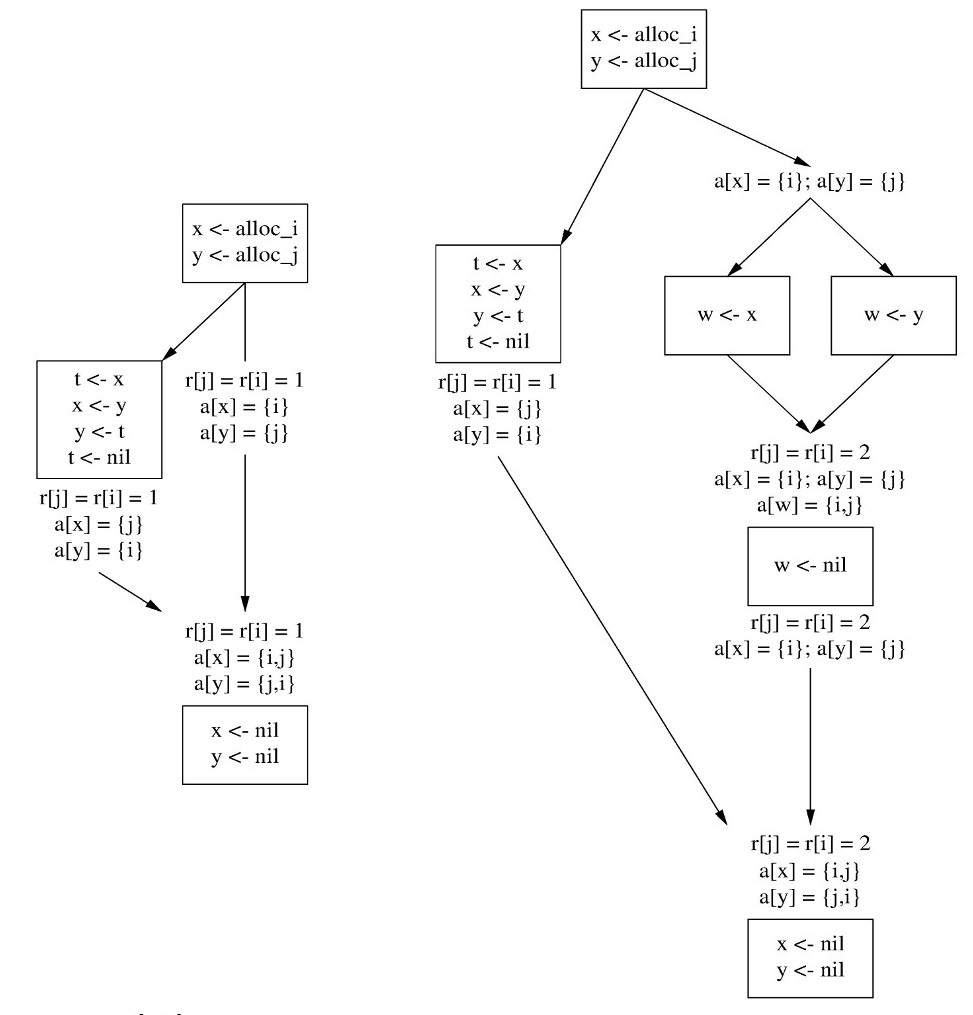
\includegraphics[height=0.79\textheight]{pic/ifgraphs_p.jpg}
  \end{center}

\end{frame}

\begin{frame}
  \frametitle{Расширение политики регионов.}
  
  \begin{block}{Политики восстановления памяти из регионов}
    \begin{itemize}
    \item Сборка мусора.
    \item Ручное управление.
    \item Замена регионов стеками.
    \item Замена регионов очередями.
    \end{itemize}
  \end{block}
\end{frame}

\begin{frame}
  \frametitle{Тестирование использования памяти.}
  
  \begin{block}{Тесты}
    \begin{itemize}
    \item Построение модели программы.
    \item Выделение всех возможных путей исполнения.
    \item Прогон каждого пути на двух моделях памяти.
    \end{itemize}
  \end{block}

  \begin{block}{Результаты}
    \begin{itemize}
    \item \textsc{Всего} выделено {\bf 22490} путей исполнения программы.
    \item \textsc{Стек стеков} потреблял меньше памяти на {\bf 226} путях.
    \item \textsc{Стек очередей} потреблял меньше памяти на {\bf 19377} путях.
    \end{itemize}
  \end{block}
\end{frame}

\begin{frame}[fragile]
  \frametitle{Предложенный язык}

  \begin{block}{Основные команды}
    \begin{itemize}
    \item \verb=enqueue(Q)= --- Поместить метку на очередь Q.
    \item \verb=dequeue(Q)= --- Удалить все объекты между началом очереди и
      первой меткой на очереди Q. 
    \item \verb=if(Q, Condition, Then, Else)= --- Выполнить, в зависимости
      от Condition, набор команд Then или Else, с локальной очередью Q.
    \item \verb=function(Qame, Q, Queues, Arguments, Body)= ---
      Создать функцию с именем Qame, основной очередью Q и аргументами
      Queues и Arguments, как последовательность команд Body.
    \end{itemize}
  \end{block}
\end{frame}

\begin{frame}[fragile]
  \frametitle{Пример программы}

\begin{verbatim}
function(fact, Q, [RQ], [V, Result],
[ if(Q1, V,                        % Если V != 0
     [ new(Q1, V1),                % Создать V1 на Q1
       sub(V, 1, V1),              % V1 = V - 1
       enqueue(Q1),                % Создать метку на Q1
       call(fact, [Q1], [V1, R1]), % Создать R1 на Q1
       dequeue(Q1),                % Освободить V1
       new(RQ, Result),            % Создать Result на RQ
       mul(R1, V, Result)          % Result = R1 * V
     ],
     [ new(RQ, Result, 1)          % Иначе Result = 1
     ])
]).
\end{verbatim}
\end{frame}

%% VOICE: ГРОМКО ТОРЖЕСТВЕННО
\begin{frame}[fragile]
  \frametitle{Результаты работы}
  \framesubtitle{}
  
  \begin{block}{Что реализовано.}
    \begin{itemize}
    \item Выделение возможных путей вычисления кода на Java.
    \item Исполнение модели программы с разными моделями памяти.
    \item Минимальный императивный язык с управлением памятью на стеке очередей.
    \end{itemize}
  \end{block}
\end{frame}

\begin{frame}
  \begin{beamercolorbox}[ht=2.5ex,dp=1ex,center,rounded=true,shadow=true]
    {frametitle}
    \usebeamerfont{frametitle}
    Спасибо за внимание
  \end{beamercolorbox}
  %% \begin{block} {Спасибо за внимание!}
  %% \end{block}
\end{frame}
\end{document}
